\section{Datenverwaltung mit Tabellenkalkulation}
\label{subsec:tables}
\subsection{Einleitung und Begriffe}
\label{subsec:EinleitungTabellen}
Daten können auf vielfältige Art und Weise festgehalten werden. Informationen über die verschiedenen Länder der Welt kann man zum Beispiel in Form eines Fliesstextes festhalten. Etwa so:

\begin{center}
    \enquote{Angola ist ein Land in Afrika, mit ungefähr 10.1 Millionen Einwohner auf einer Fläche von 1246.7 Quadratkilometern. Albanien ist ein viel kleineres Land: Seine 3.49 Millionen Einwohner verteilen sich auf 25.7 Quadratkilometern. Auch das Bruttoinlandprodukt des europäischen Landes ist mit 5.6 Milliarden USD kleiner als jenes von Angola (11.6 Milliarden) \dots }
\end{center}

Will man sich einen schnellen Überblick verschaffen oder Länder miteinander vergleichen, ist diese Art der Verwaltung von Informationen wenig effizient. Häufig ist es besser, wenn man die Daten \textbf{strukturiert}. 

Der allergrösste Teil der Daten ist in Tabellen geordnet. Eine Beispiel einer Tabelle ist gegeben in \cref{table:cia-values}.

\begin{table}[H]
  \centering
  \begin{tabular}{lcccc}
    \toprule
    \textbf{Name}    & \textbf{Region} & \textbf{Fläche [Tsd $km^2$]} & \textbf{Einwohner [Mio]} & \textbf{BIP [Mrd USD]} \\
    \midrule
    Afghanistan      & Asien           & 652             & 25.8             & 21.0        \\
    Albanien         & Europa          & 28.7            & 3.49              & 5.6         \\
    Algerien         & Afrika          & 2381.7         & 31.2              & 147.6       \\
    Amerikanische... & Ozeanien        & 0.199           & 65.4              & 0.15        \\
    Andorra          & Europa          & 0.468           & 0.67              & 1.2         \\
    Angola           & Afrika          & 1246.7         & 10.1              & 11.6        \\
    % Anguilla         & Mittelamerika   & 0.091           & 11.8K              & 0.088B       \\
    % Antarktik        & Antarktis       & 14M             & 0                  & 0            \\
    % Antigua und...   & Mittelamerika   & 0.442           & 66.4K              & 0.524B       \\
    % Argentinien      & Südamerika      & 2,766.9         & 36.9M              & 367B         \\
    \midrule
    ...              & ...             & ...             & ...                & ...          \\
    \bottomrule
  \end{tabular}
  \caption{Länder-Tabelle}
  \label{table:cia-values}
\end{table}


Eine Tabelle besteht aus Zeilen und Spalten, wie in \cref{table:table-cia} gezeigt.


\begin{table}[H]
  \centering
  \tiny
  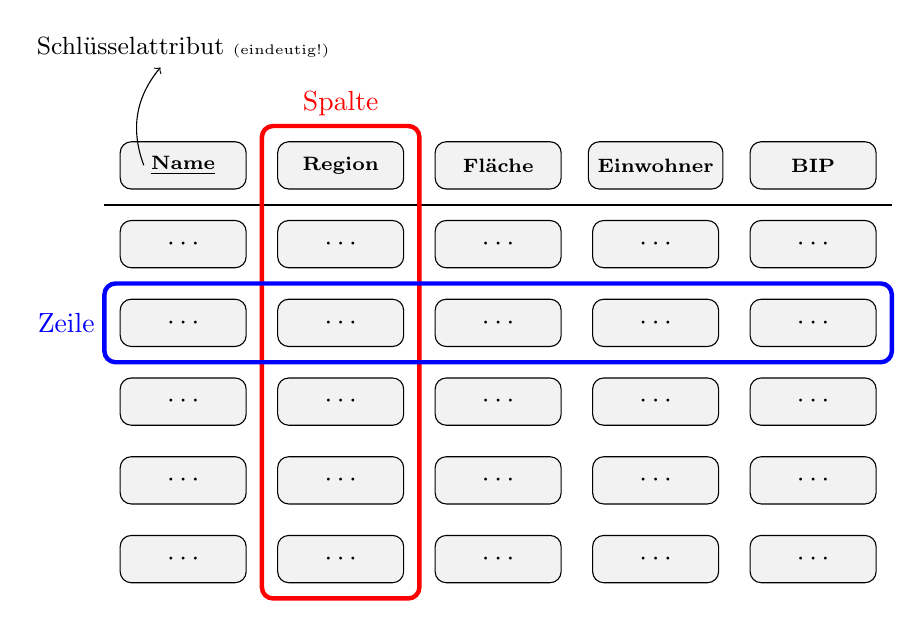
\begin{tikzpicture}
    % Define style for cell
    \tikzstyle{cell} = [draw, rectangle, minimum width=1.6cm, minimum height=.6cm, fill=gray!10, rounded corners]
    \tikzstyle{cellcdot} = [draw, rectangle, minimum width=1.6cm, minimum height=.6cm, fill=gray!0, rounded corners]

    % Draw the table
    \foreach \row in {1,...,6} {
        \foreach \col/\ctitle in {1/\underline{Name},2/Region,3/Fläche,4/Einwohner,5/BIP} {
            \node(\col\row)[cell] at (\col*2, -\row) {
              \ifnum\row=1
                \scriptsize\textbf{\ctitle}\normalsize
              \else
                $\cdots$
              \fi
            };
          }
      }
    \draw[black, thick] (1,-1.5) -- (11,-1.5);

    \draw [red,ultra thick,rounded corners]
    (3,-.5) rectangle (5,-6.5);

    \draw [blue,ultra thick,rounded corners]
    (1,-2.5) rectangle (11,-3.5);

    \node[above] at (4,-0.5){\textcolor{red}{Spalte}};
    \node[left] at (1,-3){\textcolor{blue}{Zeile}};

    \node(label) at (2,.5) {\small Schlüsselattribut \tiny(eindeutig!)};
    \path[->] (1.5,-1) edge[bend left] node [left] {} (label);
  \end{tikzpicture}
  \caption{Typische Tabellenstruktur anhand einer Tabelle mit Informationen zu Ländern}
  \label{table:table-cia}
\end{table}
In \cref{table:table-cia} enthält jede \textcolor{blue}{Zeile} Informationen zu einem Land: dessen Name, die Region (=Kontinent), Fläche, die Einwohnerzahl und das Bruttoinlandprodukt (BIP). Eine solche Zeile nennt man  einen \textbf{Datensatz} oder \textbf{Tupel}.

Jede \textcolor{red}{Spalte} enthält Informationen eines selben Typs, beispielsweise die Regionen aller Länder, die Flächen oder die Einwohnerzahlen. Die Spalten nennt man \textbf{Attribute}.

In einer Spalte sollten also alle Werte denselben \textbf{Typ} haben, beispielsweise \enquote{Zahl} (Fläche, Einwohner, BIP) oder
\enquote{Text} (Name, Region). 

Nicht zuletzt gibt es in gewissen Tabellen (genau) ein \textbf{Schlüsselattribut}, dessen Werte eindeutig sein müssen. 
Dies bedeutet in \cref{table:table-cia} beispielsweise, dass kein Ländername zweimal oder mehr vorkommen darf. Weshalb dies wichtig ist, werden wir später sehen.

\subsection{Tabellen in Excel verwalten}
\label{subsec:TabelleInExcel}

Die Informationen über die Nutzer Ihrer neuen Social Media Plattform sind auch in eine Tabelle gespeichert.

\begin{myexercise}[Tabelle users untersuchen]
    \label{myexercise:users_in_excel}
    % \begin{table}[H]
    %     \centering
    %     \begin{tabular}{r|l}
    %       \emoji{chequered-flag} & Die Tabelle users untersuchen \\\hline
    %       %\emoji{family-man-woman-girl-boy} & 3er- bis 4er-Gruppen \\\hline
    %       \emoji{student}        & Einzelarbeit                         \\\hline
    %       \emoji{stopwatch}      & ca. 5 min.
    %     \end{tabular}
    %   \end{table}
      Laden Sie die Tabelle users.xlsx von Moodle herunter und öffnen Sie sie mit Excel.
    \begin{enumerate}
        \item Wie viele Datensätze umfasst die Tabelle? Wie viele Attribute werden abgebildet?
        \item Wie viele der Nutzer sind männlich?
        \item Ist \enquote{Eleonora Walter} bereits registriert?
        \item Wie viele NutzerInnen sind grösser als 180 cm?
        \item Die Anzahl männliche Nutzer lässt sich viel leichter bestimmen, als das Vorhandensein von \enquote{Eleonora Walter} oder die Anzahl NutzerInnen, mit einer Körpergrösse über 180 cm. Was ist der Grund bzw. wie müsste man die Tabelle verändern, damit auch die beiden aufwendige Fragen einfacher zu beantworten sind?
    \end{enumerate}
\end{myexercise}



% \begin{table}
% \begin{tabular}{lllllllllllllllll}
% id&username&email&password&name&bio&gender&birthday&city&country&centimeters&avatar&role&is\_active&remember\_token&created\_at&updated\_at\\
% 1&niclas258&NiclasSchweizer@instahub.test&\$2y\$10\$VdoILxrn6CZU/PtClCDJY.eB3s0lzYiGkY7NokYpZJpMsJ2pq/tuK&Niclas Schweizer&&male&31.01.01 00:00&Wremen&Germany&182&avatars/001.jpg&user&0&&13.09.17 00:00&13.09.17 00:00\\
% 2&rafael54&RafaelProbst@instahub.test&\$2y\$10\$HkuheWgNzbw9KLo8N3kOHeM6hh7LTpLwqMOcAY7QpqKzOi7NIYqUm&Rafael Probst&&male&06.08.04 00:00&Leipzig&Germany&187&avatars/002.jpg&user&0&&22.09.17 08:32&22.09.17 08:32\\
% 3&luis52&LuisKrueger@instahub.test&\$2y\$10\$8K3Q38u2zt0lKFzwLWObBO.ZI//pt1s6MwHqsAV5qxffy8sELyHCG&Luis Krüger&&male&15.12.04 00:00&Lautertal&Germany&173&avatars/003.jpg&user&0&&26.08.17 15:00&26.08.17 15:00\\
% 4&gustav489&GustavMeister@instahub.test&\$2y\$10\$mNnEzNB4mNQ7G9vbZar4B.yI1nAsFGD/cCn1wIVZ52xueTNGo5H4K&Gustav Meister&&male&12.07.04 00:00&Halle&Germany&165&avatars/004.jpg&user&0&&20.09.17 20:28&20.09.17 20:28\\
% 5&johannes446&JohannesNadel@instahub.test&\$2y\$10\$V4l5ruRGsD99DG3dVLnHW.4ye1MinWFOqdV4WqErTw4ryR0SVEX7O&Johannes Nadel&&male&01.04.00 00:00&Leipzig&Germany&184&avatars/005.jpg&user&0&&16.09.17 21:05&16.09.17 21:05\\
% \end{tabular}
% \end{table}

% In der Tabelle der Benutzer sind Ihnen vielleicht einige Spalten aufgefallen, deren Bedeutung nicht sofort klar ist. Auf einige dieser Spalten werden wir später eingehen. Damit Sie sich aber schon einmal eine Vorstellung machen können, sollen Sie im Folgenden kurz erklärt werden.

% \begin{itemize}
%   \item Passwort: In dieser Spalte sind die Passwortinformationen der Benutzer gespeichert. Diese Passwörter sind aber nicht im Klartext abgespeichert, sondern verschlüsselt mit einer sogenannten Hash-Funktion. Damit wird sichergestellt, dass nicht einmal die Administrator*innen das echte Passwort kennen und dieses auch geheim bleibt, sollten Hacker sich Zugriff auf die Datenbank verschaffen können (Mehr dazu im Kapitel \enquote{Informationsgesellschaft}).
%   \item Bio: Die Nutzer*innen der Plattform können sich in einem kurzen Text selbst beschreiben. Bei den Nutzern, die bereits registriert sind, hat das noch niemand gemacht. Darum sind diese Felder alle leer.
%   \item Is_active: Mit diesem Eintrag können Nutzer gefunden werden, die nicht mehr aktiv sind.
% \end{itemize}

In der Tabelle sind Ihnen vielleicht die seltsamen Einträge in der Spalte password aufgefallen: Passwörter werden nicht im Klartext abgespeichert, sondern verschlüsselt mit einer sogenannten Hash-Funktion. Damit wird sichergestellt, dass nicht einmal die Administrator*innen das echte Passwort kennen und dieses auch geheim bleibt, sollten Hacker sich Zugriff auf die Datenbank verschaffen können (Mehr dazu im Kapitel \enquote{Informationsgesellschaft}).

Tabellenkalkulation-Software wie Excel bietet einige Funktionen, die Ihnen dabei helfen, Informationen aus den Tabellen zu entnehmen.

\begin{myexercise}[users als Tabelle formatieren]
  \label{myexercise:tabellenformat_in_excel}
  % \begin{table}[H]
  %     \centering
  %     \begin{tabular}{r|l}
  %       \emoji{chequered-flag} & Tabellenfunktionen in Excel kennenlernen \\\hline
  %       %\emoji{family-man-woman-girl-boy} & 3er- bis 4er-Gruppen \\\hline
  %       \emoji{student}        & Einzelarbeit                         \\\hline
  %       \emoji{stopwatch}      & ca. 10 min.
  %     \end{tabular}
  %   \end{table}
    Öffnen Sie wieder die Tabelle users.xlsx mit Excel. Falls Sie sie in der Aufgabe davor verändert haben, laden Sie sie wieder von Moodle herunter.

    Wählen Sie nun den Bereich der Tabelle aus, indem sich die Daten befinden. Mit der Tastenkombination ctrl-A oder cmd-A passiert das in der Regel automatisch. Kontrollieren Sie aber, ob nicht auch Zellen markiert wurden, die nicht zum Datenbereich gehören (in diesem Fall müssen Sie den Datenbereich von Hand markieren).

    Suchen Sie im Reiter \enquote{Start} nach dem Befehl \enquote{Als Tabelle formatieren}. Wählen Sie eine Farbkombination nach Wahl und geben Sie an, dass die Tabelle über Überschriften verfügt.

    Die Tabelle sollte nun ungefähr so aussehen:
    \begin{figure}[H]
      \centering
      \includegraphics[width=0.8\textwidth]{GrundlagenInfo/06_Datenbanken/Figures/usersAlsTabelleFormatiert.png}
    \end{figure}

    Neben den Spaltennamen sehen Sie kleine Dreiecke. Mit einem Klick auf diese Dreieck lassen sich die Daten neu Sortieren. Beantworten Sie die folgenden Fragen, indem Sie die Daten passend \textbf{sortieren}.

  \begin{enumerate}
      \item Welches ist der älteste, welches der jüngste Nutzer?
      \item Wie viele NutzerInnen sind grösser als 175 cm?
      \item Ist \enquote{Lina Drescher} bereits registriert?
      \newcounter{enumTemp}
      \setcounter{enumTemp}{\theenumi}
  \end{enumerate}

  In einigen Fällen ist es von Vorteil, wenn man nur eine Auswahl der Datensätze anzeigen lässt, die gewisse Bedingungen erfüllt. Diesen Vorgang nennt man \enquote{Filtern}. Auch die Filterfunktionen findet man, indem man auf die kleine Dreiecke in der Spaltenüberschrift klickt. Beantworten Sie die folgenden Fragen, indem Sie die Daten passend \textbf{filtern}.

  \begin{enumerate}
    \setcounter{enumi}{\theenumTemp}
    \item Filtern Sie die Tabelle, sodass nur die Nutzer aus Berlin angezeigt werden.
    \item Entfernen Sie den Filter wieder. Lassen Sie nun alle Nutzer anzeigen, die grösser als 180 cm sind.
    \item Welche weiblichen Nutzer haben eine Körpergrösse, die über dem Durchschnitt alles User liegt? 
  \end{enumerate}
  
  
\end{myexercise}

%\subsection{EVENTUELL AUCH: Aggregatfunktionen und Pivot-Tabellen}

\begin{mysummary}

\begin{itemize}
  \item Es ist häufig nützlich, Informationen in Form von \textbf{Tabellen} zu verwalten.
  \item Die Zeilen solcher Tabellen nennt man \textbf{Datensätze}, die Spalten \textbf{Attribute}.
  \item Auf der Suche man nach bestimmten Informationen lassen sich die Informationen in einer Tabellenkalkulation \textbf{sortieren} und \textbf{filtern}.
\end{itemize}
\end{mysummary}


